\chapter{Конструкторская часть}

В данном разделе будут рассмотрены схемы алгоритмов сортировок 
(блинная, перемешиванием и пирамидальная), а также найдена их трудоемкость.

\section{Разработка алгоритмов}

\begin{figure}[h]
    \centering
    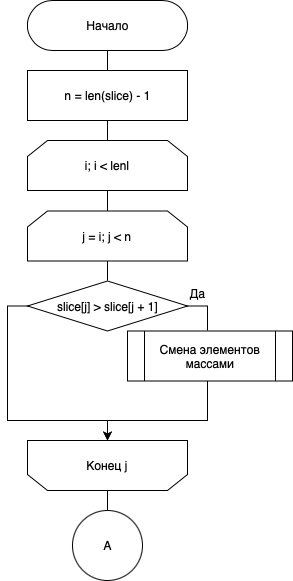
\includegraphics[width=0.4\linewidth]{img/sheker1.png}
    \caption{Схема алгоритма сортировки Перемешиванем}
    \label{fig:shecker}
\end{figure}

\begin{figure}[h]
    \centering
    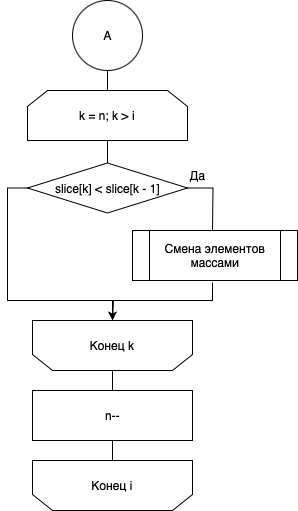
\includegraphics[width=0.4\linewidth]{img/sheker2.png}
    \caption{Схема алгоритма сортировки Перемешиванем}
    % \label{fig:shecker}
\end{figure}

\begin{figure}[h]
    \centering
    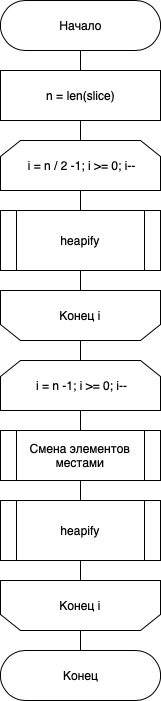
\includegraphics[width=0.2\linewidth]{img/piramid1.png}
    \caption{Схема алгоритма Пирамидальной сортировки.}
    \label{fig:piramid}
\end{figure}

\begin{figure}[h]
    \centering
    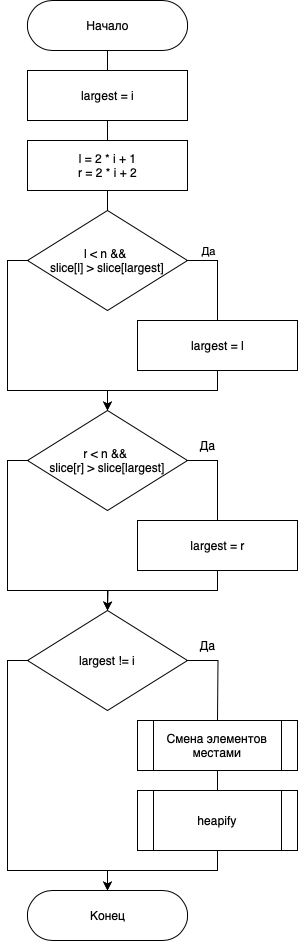
\includegraphics[width=0.4\linewidth]{img/piramid2.png}
    \caption{Схема алгоритма Пирамидальной сортировки. Функция поиска максимального.}
    % \label{fig:shecker}
\end{figure}

\begin{figure}[h]
    \centering
    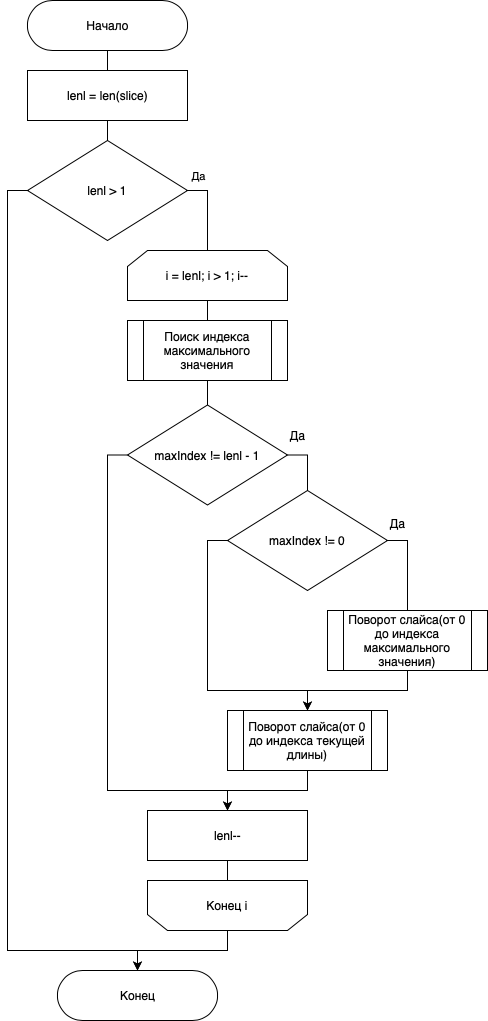
\includegraphics[width=0.5\linewidth]{img/pancake1.png}
    \caption{Схема алгоритма Блинной сортировки.}
    \label{fig:pancake}
\end{figure}

\begin{figure}[h]
    \centering
    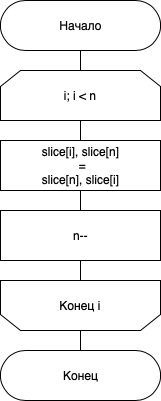
\includegraphics[width=0.2\linewidth]{img/pancake2.png}
    \caption{Схема алгоритма Блинной сортировки. Функция разворота массива}
    % \label{fig:pancake}
\end{figure}

\begin{figure}[h]
    \centering
    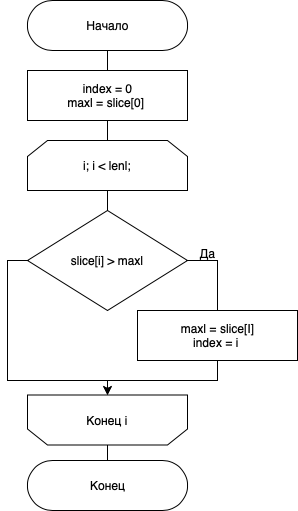
\includegraphics[width=0.4\linewidth]{img/pancake3.png}
    \caption{Схема алгоритма Блинной сортировки. Функция поиска индекса максимального значения.}
    % \label{fig:pancake}
\end{figure}

\clearpage
\section{Оценка трудоемкости алгоритмов}

В данном подразделе производится оценка трудоемкости каждого из алгоритмов.

\subsection{Модель вычислений}

Введем модель вычислений для оценки трудоемкости алгоритмов:
\begin{itemize}[left=\parindent]
    \item операции из списка \ref{op2} имеют трудоемкость 2;
        \begin{equation}\label{op2}
            *,~/,~//,~\%,~*=,~/=,~//=
        \end{equation}

    \item операции из списка \ref{op1} имеют трудоемкость 1;
        \begin{equation}\label{op1}
            \begin{aligned}
                =,~+,~-,~+=,~-=,~<,~>,~==,~!=,\\
                ~>=, ~<=,~[],~<<,~>>,~++,~--,and,or
            \end{aligned}
        \end{equation}

    \item трyдоемкость оператора выбора \texttt{if} условие \texttt{then} А
        \texttt{else} B рассчитывается по формуле \ref{ifeq}:
        \begin{equation}\label{ifeq}
            f_{if} = f_{условия} +
            \begin{cases}
                f_A, & \text{если условие выполняется;}\\
                f_B, & \text{иначе}
            \end{cases}
        \end{equation}

    \item трудоемкость оператора цикла рассчитывется по формуле \ref{foreq}:
        \begin{equation}\label{foreq}
            f_{\text{for}} = f_{\text{инициализации}} + f_{\text{сравнения}} +
                      N(f_{\text{тела}} + f_{\text{инкремента}} +
                      f_{\text{сравнения}})
        \end{equation}

    \item трyдоемкость вызова функции равна 0.
\end{itemize}

\subsection{Алгоритм сортировки перемешиванием}

В лучшем случае алгоритму подается на вход упорядоченная последовательность.
При таких входных данных первый внутренний цикл $A$ осуществлет полный проход
по последовательность в одну сторону и не находит обменов соседний элементов,
поэтому на перой же итерации внешнего цикла правая граница становится равной
левой границе, из-за чего второй внутренний цикл $B$ не отрабатывает, произведя
только ининциализацию и одну проверку условия, а внешний цикл завершает свою
работу после первой итерации. Таким образом, в лучшем случае трудоемкость
алгоритма сортировки перемешиваним равна (формула \ref{eq:bestshaker}):
\begin{equation}\label{eq:bestshaker}
    f = 4 + 1 + 2 + (N - 1)(2 + 4) + 1 + 2 + 1 + 1 =
                    6N + 6 = O(N)
\end{equation}

В худшем случае алгоритму подается на вход упорядоченная в обратном порядке
последовательность. Внешний цикл отрабатывает $\frac{N}{2}$ раз, так как за
одну итерацию на свое место ставятся 2 элемента. Количество итераций каждого
цикла зависит от четности размера подаваемой последовательнсти, если $N$ ---
четно, то цикл $A$ отработает $\frac{N - 1 + 1}{2}$ итераций, а цикл $B$ ---
$\frac{N - 2 + 1}{2}$, если $N$ --- нечетно, то цикл $A$ отработает $\frac{N -
1 + 2}{2}$ итераций, а цикл $B$ --- $\frac{N - 2}{2}$, однако и в том, и другом
случае в общем два цикла отработают $\frac{2N-1}{2}$ итераций, а так как
сложность тел обоих циклов одинаковая при вычислениях можно сразу пользоваться
общим числом итераций. Таким образом, в худшем случае трудоемкость алгоритма
сортировки перемешиванием равна (формула \ref{eq:worstshaker}):
\begin{multline}\label{eq:worstshaker}
    f = 4 + \frac{N}{2}(1 + 2 + 1 + 2 + 1 + \frac{2N-1}{2}(2 + 4 + 9
                + 1)) =\\= 4 + \frac{N}{2}(16N - 1) = 8N^2-\frac{N}{2} + 4 =
                O(N^2)
\end{multline}

\subsection{Алгоритм пирамидальной сортировки}

Трудоемкость в лучшем случае при отсортированном массиве по возрастанию выведена в формуле (\ref{сomplexity:heap_best_t}).
\begin{equation}
	\label{сomplexity:heap_best_t}
	\begin{gathered}
		f_{best} = 3 + 4 + \frac{N}{2} \cdot (2 + 1 + f_{heapify\_best}) + \\
		+ 3 + (N - 1)(2 + 2 + f_{swap} + 1 + f_{heapify\_best})
	\end{gathered}
\end{equation}

Трудоемкость в худшем случае при отсортированном массиве по убыванию выведена в формуле (\ref{сomplexity:heap_worst_t}).

\begin{equation}
	\label{сomplexity:heap_worst_t}
	\begin{gathered}
		f_{worst} = 3 + 4 + \frac{N}{2} \cdot (2 + 1 + f_{heapify\_worst}) + \\
		+ 3 + (N - 1)(2 + 2 + f_{swap} + 1 + f_{heapify\_worst})
	\end{gathered}
\end{equation}

Трудоемкость перестановки элементов будет равна, формула (\ref{сomplexity:swap})
\begin{equation}
	\label{сomplexity:swap}
	f_{swap} = 6
\end{equation}

Трудоемкость части программы сортировки пирамиды является функция heapify.

\begin{equation}
	\label{сomplexity:heapify_best}
	f_{heapify\_best} = 5 + log N \cdot (5 + 3 + 4 + 2 + 4) = 5 + 17 \cdot log N = O(log N) 
\end{equation}

\begin{equation}
	\label{сomplexity:heapify_worst}
	f_{heapify\_worst} = 5 + log N \cdot (5 + 3 + 4 + 5 + 7) = 5 + 24 \cdot log N = O(log N) 
\end{equation}

Исходя из выведенных выше, то лучший и худший случаи будут равны: 

\begin{equation}
	\label{сomplexity:heap_best_p}
	\begin{gathered}
		f_{best} = 7 + \frac{N}{2} \cdot (3 + 5 + 17 \cdot log N) + 3 + (N - 1) \cdot (5 + 6 + \\ 
		+ 5 + 17 \cdot log N) = 23N + 24N \cdot log N - 13 \cdot log N - 3 =\\
		= O(N \cdot log N)
	\end{gathered}
\end{equation}

\begin{equation}
	\label{сomplexity:heap_worst_p}
	\begin{gathered}
		f_{worst} = 7 + \frac{N}{2} \cdot (3 + 5 + 24 \cdot log N) + 3 + (N - 1) \cdot (5 + 6 + \\ 
		+ 5 + 24 \cdot log N) = 23N + 33N \cdot log N - 24 \cdot log N - 3 =\\
		= O(N \cdot log N)
	\end{gathered}
\end{equation}

Таким образов из выведенных результатов в формулах (\ref{сomplexity:heap_best_p}) и (\ref{сomplexity:heap_worst_p}) можно понять, что лучший и худший случай имеют трудоемкость $O(N \cdot log N)$.

\subsection{Алгоритм блинной сортировки}

Трудоемкость в случае, если элементы массива расположены в произвольном порядке.
\begin{equation}
    \label{сomplexity:pancake1}
    \begin{gathered}
        f_{worst} = 1 + 1 + 2 + N(2 + f_{searchMaxIndex} + 2 + 1 + f_{flipSlice} * 2)
    \end{gathered}
\end{equation}

Трудоемкость в случае, если массив отсортирован по убыванию.
\begin{equation}
    \label{сomplexity:pancake2}
    \begin{gathered}
        f_{middle} = 1 + 1 + 2 + N(2 + f_{searchMaxIndex} + 2 + 1 + f_{flipSlice})
    \end{gathered}
\end{equation}

Трудоемкость в случае, если массив отсортирован по возрастанию.
\begin{equation}
    \label{сomplexity:pancake3}
    \begin{gathered}
        f_{best} = 1 + 1 + 2 + N(2 + f_{searchMaxIndex} + 2)
    \end{gathered}
\end{equation}

Рассмотрим трудоемкость функции searchMaxIndex.
\begin{equation}
    \label{сomplexity:searchMaxIndex}
    \begin{gathered}
        f_{searchMaxIndex} = 3 + 2 + N(2 + 2 + 2 + 1) = 5 + 7N
    \end{gathered}
\end{equation}

Рассмотрим трудоемкость функции flipSlice.
\begin{equation}
    \label{сomplexity:flipSlice}
    \begin{gathered}
        f_{flipSLice} = 2 + N(2 + 6 + 1) = 2 + 9N
    \end{gathered}
\end{equation}

Добавляя трудоемкости функций (\ref{сomplexity:searchMaxIndex}) и (\ref{сomplexity:flipSlice}) в формулы
(\ref{сomplexity:pancake1}), (\ref{сomplexity:pancake2}), (\ref{сomplexity:pancake3}) получим:

Трудоемкость в случае, если элементы массива расположены в произвольном порядке.
\begin{equation}
    \label{сomplexity:pancake1}
    \begin{gathered}
        f_{worst} = 1 + 1 + 2 + N(2 + 5 + 7N + 2 + 1 + (2 + 9N) * 2) = \\
            = 4 + N(14 + 25N) = 25N^2 + 14N + 4 = O(N^2)
    \end{gathered}
\end{equation}

Трудоемкость в случае, если массив отсортирован по убыванию.
\begin{equation}
    \label{сomplexity:pancake2}
    \begin{gathered}
        f_{middle} = 1 + 1 + 2 + N(2 + 5 + 7N + 2 + 1 + 2 + 9N = \\
            = 4 + N(12 + 16N) = 16N^2 + 12N + 4 = O(N^2)
    \end{gathered}
\end{equation}

Трудоемкость в случае, если массив отсортирован по возрастанию.
\begin{equation}
    \label{сomplexity:pancake3}
    \begin{gathered}
        f_{best} = 1 + 1 + 2 + N(2 + 5 + 7N + 2) = \\
            = 3 + N(9 + 7N) = 7N^2 + 9N + 3 = O(N^2)
    \end{gathered}
\end{equation}

\section{Описание используемых типов данных}

При реализации алгоритмов будут использованы следующие структуры данных:

\begin{itemize}
	\item длина массива --- целое число;
	\item массив --- набор целых чисел;
\end{itemize}

\section{Требования к ПО}
Программа должна предоставлять следующие возможности:
\begin{itemize}[left=\parindent]
    \item выбор режима работы: единичный эксперимент и замер времени работы алгоритмов сортировки;
    \item в режиме единичного эксперимента ввод размеров и содержимого сортируемого массив;
    \item в режиме замера времени происходит замер времени при различных
          размерах матриц и различных видах отсортированности(по убыванию, по возрастанию, рандомно).
\end{itemize}

\section*{Вывод}

В данном разделе были разработаны алгоритмы сортировки блинная,
перемешиванием и пирамидальная, также была произведена оценка трудоемкостей
алгоритмов.